\documentclass[tikz,border=2pt]{standalone}

\usepackage[T1]{fontenc}
\usepackage{amsmath,amssymb}
\usepackage{graphicx}
\usepackage{xcolor}
\usetikzlibrary{arrows.meta,calc,positioning}
\graphicspath{{figures/}}

\definecolor{ink}{HTML}{111827}
\definecolor{muted}{HTML}{4B5563}
\definecolor{linegray}{HTML}{9CA3AF}
\definecolor{condition}{HTML}{4C78A8}
\definecolor{fusion}{HTML}{0F766E}
\definecolor{network}{HTML}{D97706}
\definecolor{wavelet}{HTML}{8B5CF6}
\definecolor{objective}{HTML}{54A24B}

\tikzset{
  panel/.style={
    draw=#1,
    fill=#1!3,
    rounded corners=3pt,
    line width=0.7pt,
  },
  block/.style={
    draw=ink!75,
    fill=white,
    rounded corners=2pt,
    line width=0.55pt,
    align=center,
    inner xsep=4pt,
    inner ysep=3pt,
    minimum height=0.72cm,
  },
  conditionblock/.style={block,draw=condition,fill=condition!7},
  fusionblock/.style={block,draw=fusion,fill=fusion!7},
  networkblock/.style={block,draw=network,fill=network!7},
  waveletblock/.style={block,draw=wavelet,fill=wavelet!7},
  lossblock/.style={block,draw=objective,fill=objective!7},
  imageblock/.style={
    draw=#1,
    fill=white,
    rounded corners=2pt,
    line width=0.65pt,
    align=center,
    inner sep=2pt,
  },
  operator/.style={
    draw=ink!65,
    fill=ink!3,
    rounded corners=2pt,
    line width=0.5pt,
    align=center,
    inner xsep=3pt,
    inner ysep=2.5pt,
    minimum height=0.58cm,
  },
  arrow/.style={
    -{Latex[length=0.9mm,width=0.68mm]},
    draw=ink,
    line width=0.65pt,
    shorten <=0.35pt,
    shorten >=0.35pt,
  },
  softarrow/.style={arrow,draw=muted},
  finalarrow/.style={arrow,dashed,draw=fusion},
  note/.style={align=center,text=muted,font=\scriptsize},
  dimension/.style={align=center,text=muted,font=\scriptsize},
}

\begin{document}
\begin{tikzpicture}[x=1cm,y=1cm,font=\footnotesize,text=ink]

% Shared conditioning column.
\draw[panel=condition] (0,0) rectangle (4.55,10.10);
\node[font=\small\bfseries,text=condition] at (2.275,9.80)
  {(a) Shared conditioning};
\node[font=\bfseries,text=condition] at (2.275,9.34)
  {Condition preparation};

\node[imageblock=condition] (xv) at (0.83,8.35)
  {\begin{tabular}{@{}c@{}}
     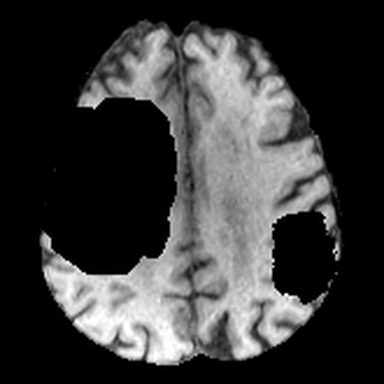
\includegraphics[width=0.70cm]{catch_architecture_voided}\\[1pt]
     \scriptsize Voided $x_v$
   \end{tabular}};
\node[operator,minimum width=0.82cm,right=0.15cm of xv] (dwtv)
  {Haar\\DWT};
\node[conditionblock,font=\scriptsize,minimum width=1.32cm,inner xsep=2pt,
  right=0.12cm of dwtv] (cv)
  {$c_v=\mathcal W(x_v)$\\$8\!\times\!128^3$};
\draw[arrow] (xv) -- (dwtv);
\draw[arrow] (dwtv) -- (cv);

\node[imageblock=condition] (mask) at (0.83,6.55)
  {\begin{tabular}{@{}c@{}}
     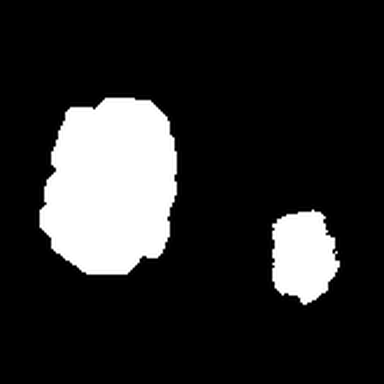
\includegraphics[width=0.70cm]{catch_architecture_mask}\\[1pt]
     \scriptsize Mask $m$
   \end{tabular}};
\node[operator,minimum width=1.18cm,right=0.15cm of mask] (maskmap)
  {nearest $\downarrow$\\$2m-1$};
\node[conditionblock,minimum width=1.12cm,right=0.15cm of maskmap] (signed)
  {$s$\\$1\!\times\!128^3$};
\draw[arrow] (mask) -- (maskmap);
\draw[arrow] (maskmap) -- (signed);

\draw[linegray,line width=0.45pt] (0.30,5.30) -- (4.25,5.30);
\node[font=\bfseries,text=fusion] at (2.275,4.98) {Concatenation};
\node[fusionblock,text width=3.24cm,inner ysep=4pt] (sharedfusion)
  at (2.275,4.10)
  {$F_{\mathrm{concat}}(z_t,c_v,s)$\\[1pt]
   $=[z_t\,\|\,c_v\,\|\,s]$};
\node[dimension] at (2.275,3.37)
  {$8+8+1=17$ channels at $128^3$};
\node[conditionblock,font=\scriptsize,minimum width=1.45cm,inner ysep=2pt]
  (sharedcond) at (2.275,2.35) {shared $c_v,s$};
\node[lossblock,font=\scriptsize,text width=1.15cm,inner xsep=2pt,inner ysep=2pt]
  (trainuse) at (1.22,1.05) {training (b)};
\node[fusionblock,font=\scriptsize,text width=1.40cm,inner xsep=2pt,inner ysep=2pt]
  (inferuse) at (3.30,1.05) {inference (c)\\five seeds};
\coordinate (sharedfork) at (2.275,1.59);
\draw[draw=muted,line width=0.65pt] (sharedcond.south) -- (sharedfork);
\draw[softarrow,shorten <=0pt] (sharedfork) -| (trainuse.north);
\draw[softarrow,shorten <=0pt] (sharedfork) -| (inferuse.north);

% Training panel.
\draw[panel=objective] (4.80,5.65) rectangle (15.50,10.10);
\node[font=\small\bfseries,text=objective] at (10.15,9.80) {(b) Training};

\node[imageblock=objective] (trainx) at (5.75,8.70)
  {\begin{tabular}{@{}c@{}}
     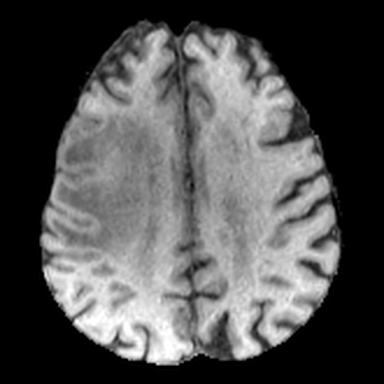
\includegraphics[width=0.64cm]{catch_architecture_complete}\\[1pt]
     \scriptsize Complete $x$
   \end{tabular}};
\node[operator,minimum width=0.76cm,right=0.20cm of trainx] (traindwt)
  {Haar\\DWT};
\node[waveletblock,minimum width=1.02cm,right=0.20cm of traindwt] (zclean)
  {clean $z_0$\\$8\!\times\!128^3$};
\node[operator,minimum width=1.08cm,right=0.20cm of zclean] (forward)
  {noise at $t$\\$q(z_t\mid z_0)$};
\node[waveletblock,minimum width=0.98cm,right=0.20cm of forward] (znoisy)
  {noisy $z_t$\\$8\!\times\!128^3$};

\node[fusionblock,minimum width=1.18cm] (trainfusion) at (7.20,6.95)
  {$F_{\mathrm{concat}}$};
\node[networkblock,text width=2.00cm,font=\scriptsize,inner xsep=2pt,inner ysep=2pt,
  right=0.20cm of trainfusion] (trainnet)
  {\textbf{3D WavUNet} $D_\theta$\\[-1pt]
   HF Haar skips\\[-1pt]
   $t$-ResBlocks};
\node[waveletblock,minimum width=1.10cm,right=0.20cm of trainnet] (zpred)
  {predicted $\hat z_0$\\$8\!\times\!128^3$};
\node[lossblock,text width=2.50cm,font=\scriptsize,inner xsep=2pt,inner ysep=1pt,
  right=0.30cm of zpred] (loss)
  {training loss\\[-1pt]
   $\mathcal L=\mathcal L_{\mathrm{wav}}$\\[-1pt]
   $+\,10\mathcal L_{\mathrm{mask}}$};

\draw[arrow] (trainx) -- (traindwt);
\draw[arrow] (traindwt) -- (zclean);
\draw[arrow] (zclean) -- (forward);
\draw[arrow] (forward) -- (znoisy);
\draw[arrow] (znoisy.south) -- ++(0,-0.34) -| (trainfusion.north);
\draw[arrow] (trainfusion) -- (trainnet);
\draw[arrow] (trainnet) -- (zpred);
\draw[arrow] (zpred) -- (loss);
\draw[softarrow] (zclean.south) -- ++(0,-0.27) -- (6.00,8.03)
  -- (6.00,6.07) -| (loss.south);
\node[note,fill=objective!3,inner sep=1pt] at (10.75,5.99)
  {clean target $z_0$};

% Inference panel.
\draw[panel=fusion] (4.80,0) rectangle (15.50,5.40);
\node[font=\small\bfseries,text=fusion] at (10.15,5.12)
  {(c) Inference: reverse sampling and $N=5$ aggregation};
\node[note] at (10.15,4.78)
  {One EMA checkpoint; five case-stable noise seeds.};

\node[waveletblock,text width=1.08cm,font=\scriptsize,inner xsep=2pt]
  (noise) at (5.58,3.82) {$z_T^{(i)}$\\$\sim\mathcal N(0,I)$};
\node[waveletblock,text width=0.90cm,font=\scriptsize,inner xsep=2pt,
  right=0.18cm of noise] (current) {current\\$z_t$};
\node[fusionblock,text width=1.00cm,font=\scriptsize,inner xsep=2pt,
  right=0.18cm of current] (inferfusion) {$F_{\mathrm{concat}}$};
\node[networkblock,text width=1.48cm,font=\scriptsize,inner xsep=2pt,inner ysep=2pt,
  right=0.18cm of inferfusion] (infernet)
  {\textbf{3D WavUNet} $D_\theta$\\[-1pt]
   HF Haar skips\\[-1pt]
   $t$-ResBlocks};
\node[waveletblock,text width=1.16cm,font=\scriptsize,inner xsep=2pt,
  right=0.18cm of infernet] (inferpred) {predicted\\$\hat z_0$};
\node[operator,text width=1.65cm,font=\scriptsize,inner xsep=2pt,
  right=0.18cm of inferpred] (posterior)
  {DDPM posterior\\$p(z_{t-1}\mid z_t,\hat z_0)$};
\node[waveletblock,text width=0.64cm,font=\scriptsize,inner xsep=2pt,
  right=0.18cm of posterior] (next) {$z_{t-1}$};

\draw[arrow] (noise) -- (current);
\draw[arrow] (current) -- (inferfusion);
\draw[arrow] (inferfusion) -- (infernet);
\draw[arrow] (infernet) -- (inferpred);
\draw[arrow] (inferpred) -- (posterior);
\draw[arrow] (posterior) -- (next);
\draw[softarrow] (next.south) -- ++(0,-0.58) -| (current.south);
\node[note,fill=fusion!3,inner sep=1pt] at (10.15,2.65)
  {repeat independently for five seeds, $t=T,\ldots,2$};

\node[waveletblock,text width=1.16cm,font=\scriptsize,inner xsep=2pt]
  (finalz) at (5.58,0.94)
  {five final states\\$\{z_0^{(i)}\}_{i=1}^{5}$};
\node[operator,text width=1.25cm,font=\scriptsize] (decode) at (7.12,0.94)
  {Haar IDWT\\$+$ hard composite};

\foreach \i/\yy in {1/1.60,2/1.26,3/0.92,4/0.58,5/0.24} {
  \node[block,draw=fusion,fill=fusion!6,minimum width=0.78cm,
    minimum height=0.21cm,inner xsep=1pt,inner ysep=0.4pt,font=\scriptsize]
    (member\i) at (8.62,\yy) {$\hat x^{(\i)}$};
  \draw[draw=muted,line width=0.55pt] (decode.east) -- (member\i.west);
}
\node[note,text=fusion] at (8.62,1.98) {five reconstructions};
\coordinate (merge) at (9.38,0.92);
\foreach \i in {1,...,5} {
  \draw[draw=muted,line width=0.55pt] (member\i.east) -- (merge);
}
\fill[fusion] (merge) circle (0.8pt);

\node[fusionblock,text width=1.18cm,font=\scriptsize] (aggregate) at (10.46,0.94)
  {voxel-wise mean\\$\bar x=\frac{1}{5}\sum_i\hat x^{(i)}$};
\node[fusionblock,text width=1.26cm,font=\scriptsize] (composite) at (12.38,0.94)
  {final hard composite\\with $x_v,m$};
\node[block,draw=fusion,fill=fusion!12,minimum width=0.98cm,font=\scriptsize]
  (output) at (14.42,0.94) {$N=5$\\prediction};

\draw[finalarrow] (next.east) -- (15.27,3.82) -- (15.27,2.24)
  -- node[midway,above,fill=fusion!3,inner sep=1.2pt,
    font=\scriptsize,text=fusion] {at $t=1$: retain five states}
  (5.58,2.24) -- (finalz.north);
\draw[arrow] (finalz) -- (decode);
\draw[softarrow] (merge) -- (aggregate);
\draw[arrow] (aggregate) -- (composite);
\draw[arrow] (composite) -- (output);

\end{tikzpicture}
\end{document}
